%%%%%%%%%%%%%%%%%%%%%%%%%%%%%%%%%%%%%%%%%%%%%%%%%%%%%%%%%%%%%%%%%%%%%%
%%  Copyright by Wenliang Du.                                       %%
%%  This work is licensed under the Creative Commons                %%
%%  Attribution-NonCommercial-ShareAlike 4.0 International License. %%
%%  To view a copy of this license, visit                           %%
%%  http://creativecommons.org/licenses/by-nc-sa/4.0/.              %%
%%%%%%%%%%%%%%%%%%%%%%%%%%%%%%%%%%%%%%%%%%%%%%%%%%%%%%%%%%%%%%%%%%%%%%

\newcommand{\devtoolFigs}{../Web_Common/Figs}


% -------------------------------------------
% SUBSECTION
% ------------------------------------------- 
\subsection{Using the \texttt{"HTTP Header Live"} add-on to Inspect HTTP Headers}
\label{web:sec:httpheaderlive}


The version of Firefox (version 60) in our Ubuntu 16.04 VM does not support the
\texttt{LiveHTTPHeader} add-on, which was used in our Ubuntu 12.04 VM. 
A new add-on called \texttt{"HTTP Header Live"} is used in its place. 
The instruction on how to enable and use this add-on tool
is depicted in Figure~\ref{web:fig:httpheader}. Just click the icon marked
by \ding{192}; a sidebar will show up on the left. Make sure that
\texttt{HTTP Header Live} is selected at position \ding{193}. Then click
any link inside a web page, all the triggered HTTP requests will be
captured and displayed inside the sidebar area marked by \ding{194}.
If you click on any HTTP request, a pop-up window will show up to display
the selected HTTP request. Unfortunately, there is a bug in this add-on
tool (it is still under development); nothing will show up inside the
pop-up window unless you change its size~(It seems that re-drawing
is not automatically triggered when the window pops up, but changing its
size will trigger the re-drawing).


\begin{figure}[htb]
\begin{center}
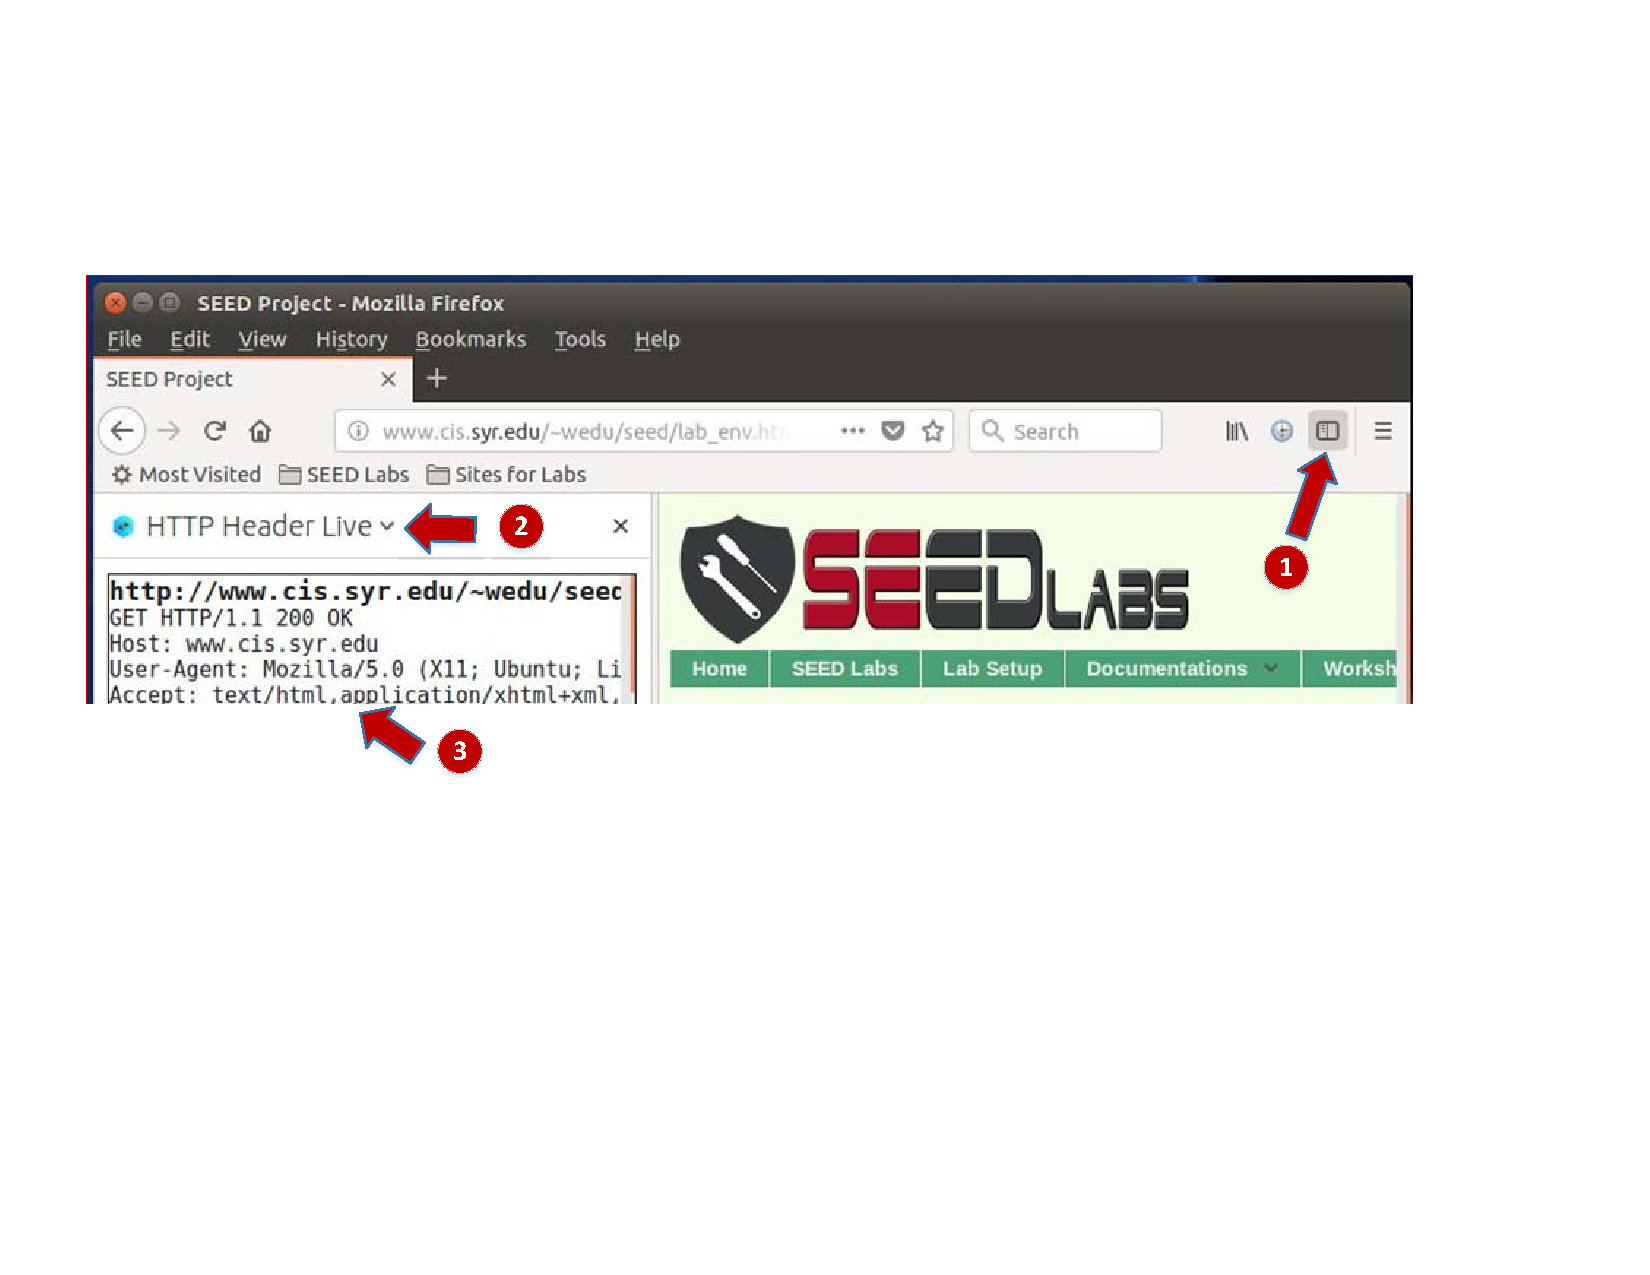
\includegraphics[width=0.85\textwidth]{\devtoolFigs/HTTPHeaderLive.pdf}
\end{center}
\caption{Enable the HTTP Header Live Add-on}
\label{web:fig:httpheader}
\end{figure}




% -------------------------------------------
% SUBSECTION
% ------------------------------------------- 
\subsection{Using the Web Developer Tool to Inspect HTTP Headers}
\label{web:sec:web_dev_tools}


There is
another tool provided by Firefox that can be quite useful 
in inspecting HTTP headers. 
The tool is the Web Developer Network Tool.  In this
section, we cover some of the important features of the tool. 
The Web Developer Network Tool can be enabled via the following navigation: 


\begin{lstlisting}
Click Firefox's top right menu --> Web Developer --> Network
 or 
Click the "Tools" menu --> Web Developer --> Network 
\end{lstlisting}


We use the user login page in Elgg as an example. 
Figure~\ref{fig:webdevtools_01_request} shows the Network Tool showing the HTTP POST request
that was used for login.

\begin{figure}[htb]
\begin{center}
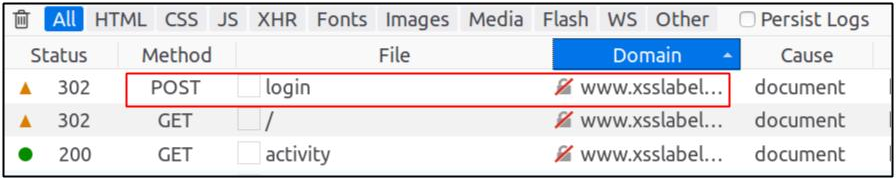
\includegraphics[width=0.8\textwidth]{\devtoolFigs/webdevtools_01_request.png}
\end{center}
\caption{HTTP Request in Web Developer Network Tool}
\label{fig:webdevtools_01_request}
\end{figure}

To further see the details of the request, we can click on a particular HTTP request and the
tool will show the information in two panes (see Figure~\ref{fig:webdevtools_02_two_panes}). 

\begin{figure}[htb]
\begin{center}
	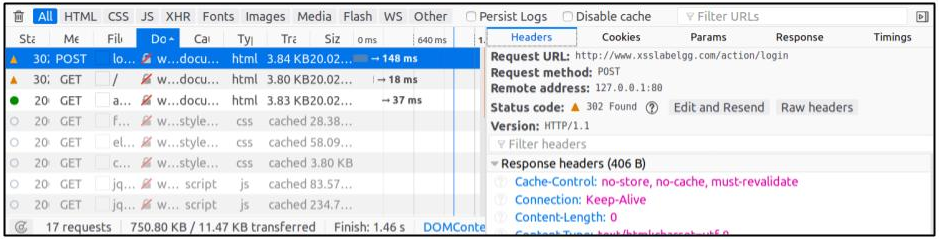
\includegraphics[width=0.95\textwidth]{\devtoolFigs/webdevtools_02_two_panes.png}
\end{center}
\caption{HTTP Request and Request Details in Two Panes}
\label{fig:webdevtools_02_two_panes}
\end{figure}



The details of the selected request will be visible in the right pane.
Figure~\ref{fig:webdevtools_03_post_headers} shows the details of the login request in the
\texttt{Headers} tab (details include URL, request method, and cookie). One can observe both
request and response headers in the right pane. To check the parameters involved in an HTTP
request, we can use the \texttt{Params} tab. Figure~\ref{fig:webdevtools_03_post_params} shows
the parameter sent in the login request to Elgg, including \texttt{username} and
\texttt{password}. The tool can be used to inspect HTTP GET requests in a similar manner to HTTP POST requests.

\begin{figure}[htb]
 \centering
 \subfigure[HTTP Request Headers]{
        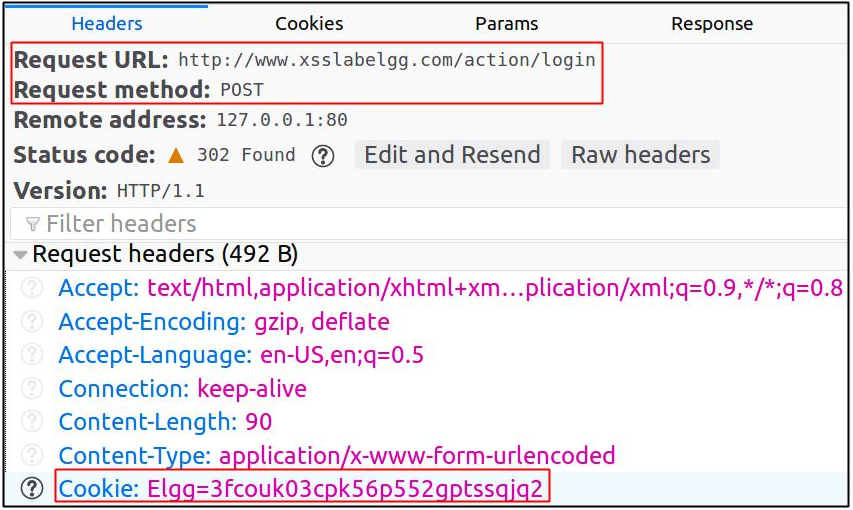
\includegraphics[width=0.6\textwidth]{\devtoolFigs/webdevtools_03-1.png}
        \label{fig:webdevtools_03_post_headers}
 }
 \subfigure[HTTP Request Parameters]{
        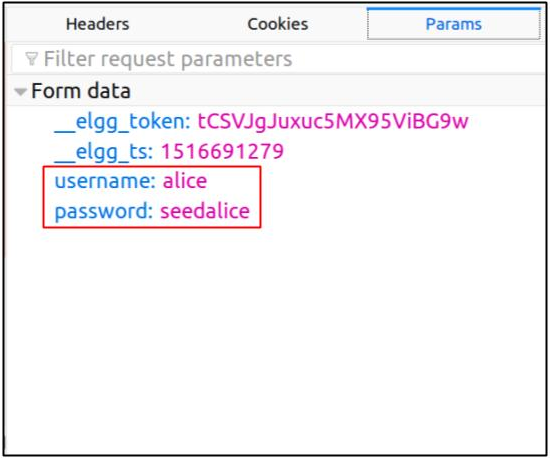
\includegraphics[width=0.35\textwidth]{\devtoolFigs/webdevtools_03-2.png}
        \label{fig:webdevtools_03_post_params}
 }
 \caption{HTTP Headers and Parameters}
\end{figure}


\paragraph{Font Size.} The default font size of Web Developer Tools window is quite small. It
can be increased by focusing click anywhere in the Network Tool window, and then using
\texttt{Ctrl} and \texttt{+} button.


% -------------------------------------------
% SUBSECTION
% -------------------------------------------
\subsection{JavaScript Debugging}
\label{web:sec:jsdebugging}

We may also need to debug our JavaScript code. Firefox's Developer Tool can also help debug
JavaScript code. It can point us to the precise places where errors occur. The following
instruction shows how to enable this debugging tool:

\begin{lstlisting}
 Click the "Tools" menu --> Web Developer --> Web Console
 or use the Shift+Ctrl+K shortcut.
\end{lstlisting}


Once we are in the web console, click the {\tt JS} tab. Click the downward pointing arrowhead
beside {\tt JS} and ensure there is a check mark beside {\tt Error}. If you are also interested
in Warning messages, click {\tt Warning}. See Figure~\ref{devtool:fig:errocheckmark}.


\begin{figure}[htb]
\begin{center}
  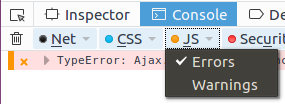
\includegraphics[width=0.4\textwidth]{\devtoolFigs/errorCheckMark.png}
\end{center}
\caption{Debugging JavaScript Code (1)}
\label{devtool:fig:errocheckmark}
\end{figure}
 

If there are any errors in the code, a message will display in the console. The line that
caused the error appears on the right side of the error message in the console. Click on the
line number and you will be taken to the exact place that has the error.
See Figure~\ref{devtool:fig:console}.


\begin{figure}[htb]
\begin{center}
  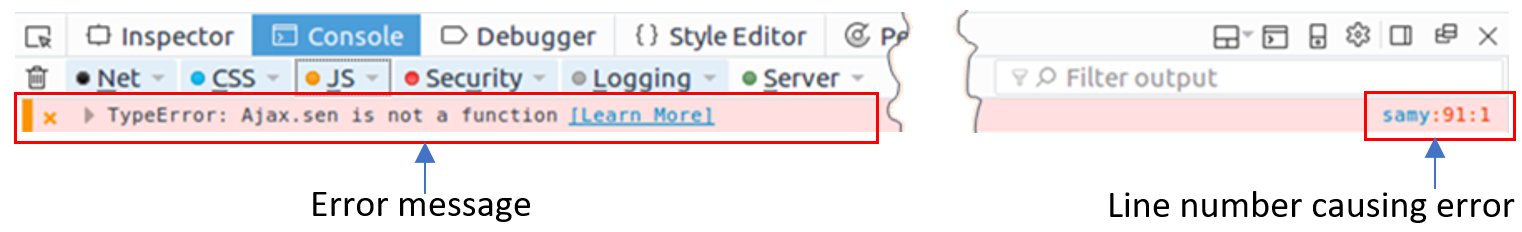
\includegraphics[width=1.0\textwidth]{\devtoolFigs/consoleError2.png}
\end{center}
\caption{Debugging JavaScript Code (2)}
\label{devtool:fig:console}
\end{figure}
 




 
